\newsavebox{\resultspanels}
\begin{lrbox}{\resultspanels}
\begin{minipage}{\textwidth}
\captionsetup{hypcap=false}
\centering
\begin{minipage}[c]{0.49\textwidth}
\footnotesize
\setlength{\tabcolsep}{2pt}
\renewcommand{\arraystretch}{1.0}
\centering
\captionsetup{font=footnotesize}
\captionof{table}{Comparison of \textbf{Unified EB} vs.\ \textbf{RES} across benchmarks ($\text{EB}=0.1, \text{max\_dns}=48$). Scores report \textbf{Avg@20} $\pm$ 95\% CI (Pass@1 averaged across 20 seeds; 5 seeds for LiveCodeBench). Relative TPF deltas are shown underneath.}
\label{tab:eb_unified_vs_rolling}
\vspace{4pt}
\begin{tabular*}{\linewidth}{@{\extracolsep{\fill}}lcccc@{}}
\toprule
& \multicolumn{2}{c}{\textbf{Unified EB}} & \multicolumn{2}{c}{\textbf{RES}} \\
\cmidrule(lr){2-3} \cmidrule(lr){4-5}
\textbf{Task} & \textbf{Avg@20} & \textbf{TPF} & \textbf{Avg@20} & \textbf{TPF} \\
\midrule
LiveCodeBench & \begin{tabular}[t]{@{}c@{}}65.4\% \\ \scriptsize{($\pm$3.2\%)}\end{tabular} & 18.7 & \begin{tabular}[t]{@{}c@{}}62.6\% \\ \scriptsize{($\pm$3.2\%)}\end{tabular} & \begin{tabular}[t]{@{}c@{}}\textbf{26.3} \\ \scriptsize{(+40.6\%)}\end{tabular} \\
\addlinespace[2pt]
Natural2Code & \begin{tabular}[t]{@{}c@{}}\textbf{93.0\%} \\ \scriptsize{\textbf{($\pm$0.8\%)}}\end{tabular} & 22.9 & \begin{tabular}[t]{@{}c@{}}91.3\% \\ \scriptsize{($\pm$0.9\%)}\end{tabular} & \begin{tabular}[t]{@{}c@{}}\textbf{30.1} \\ \scriptsize{(+31.7\%)}\end{tabular} \\
\addlinespace[2pt]
GPQA Diamond & \begin{tabular}[t]{@{}c@{}}67.5\% \\ \scriptsize{($\pm$1.5\%)}\end{tabular} & 16.6 & \begin{tabular}[t]{@{}c@{}}68.3\% \\ \scriptsize{($\pm$1.4\%)}\end{tabular} & \begin{tabular}[t]{@{}c@{}}\textbf{23.8} \\ \scriptsize{(+43.1\%)}\end{tabular} \\
\addlinespace[2pt]
HiddenMath   & \begin{tabular}[t]{@{}c@{}}\textbf{73.9\%} \\ \scriptsize{\textbf{($\pm$0.9\%)}}\end{tabular} & 22.1 & \begin{tabular}[t]{@{}c@{}}72.6\% \\ \scriptsize{($\pm$0.9\%)}\end{tabular} & \begin{tabular}[t]{@{}c@{}}\textbf{27.2} \\ \scriptsize{(+23.2\%)}\end{tabular} \\
\addlinespace[2pt]
GSM8k        & \begin{tabular}[t]{@{}c@{}}\textbf{92.1\%} \\ \scriptsize{\textbf{($\pm$0.3\%)}}\end{tabular} & 21.7 & \begin{tabular}[t]{@{}c@{}}91.6\% \\ \scriptsize{($\pm$0.3\%)}\end{tabular} & \begin{tabular}[t]{@{}c@{}}\textbf{27.7} \\ \scriptsize{(+28.0\%)}\end{tabular} \\
\addlinespace[2pt]
IFEval       & \begin{tabular}[t]{@{}c@{}}\textbf{93.1\%} \\ \scriptsize{\textbf{($\pm$0.5\%)}}\end{tabular} & 16.8 & \begin{tabular}[t]{@{}c@{}}82.4\% \\ \scriptsize{($\pm$0.7\%)}\end{tabular} & \begin{tabular}[t]{@{}c@{}}\textbf{22.6} \\ \scriptsize{(+34.4\%)}\end{tabular} \\
\addlinespace[2pt]
MMLU         & \begin{tabular}[t]{@{}c@{}}80.3\% \\ \scriptsize{($\pm$0.4\%)}\end{tabular} & 16.2 & \begin{tabular}[t]{@{}c@{}}\textbf{82.8\%} \\ \scriptsize{\textbf{($\pm$0.4\%)}}\end{tabular} & \begin{tabular}[t]{@{}c@{}}\textbf{21.0} \\ \scriptsize{(+30.0\%)}\end{tabular} \\
\midrule
\textbf{Macro Average} & \begin{tabular}[t]{@{}c@{}}\textbf{80.7\%} \\ \scriptsize{\textbf{($\pm$0.5\%)}}\end{tabular} & 19.3 & \begin{tabular}[t]{@{}c@{}}78.8\% \\ \scriptsize{($\pm$0.5\%)}\end{tabular} & \begin{tabular}[t]{@{}c@{}}\textbf{25.5} \\ \scriptsize{\textbf{(+32.5\%)}}\end{tabular} \\
\bottomrule
\end{tabular*}



\end{minipage}\hfill
\begin{minipage}[c]{0.49\textwidth}
\centering
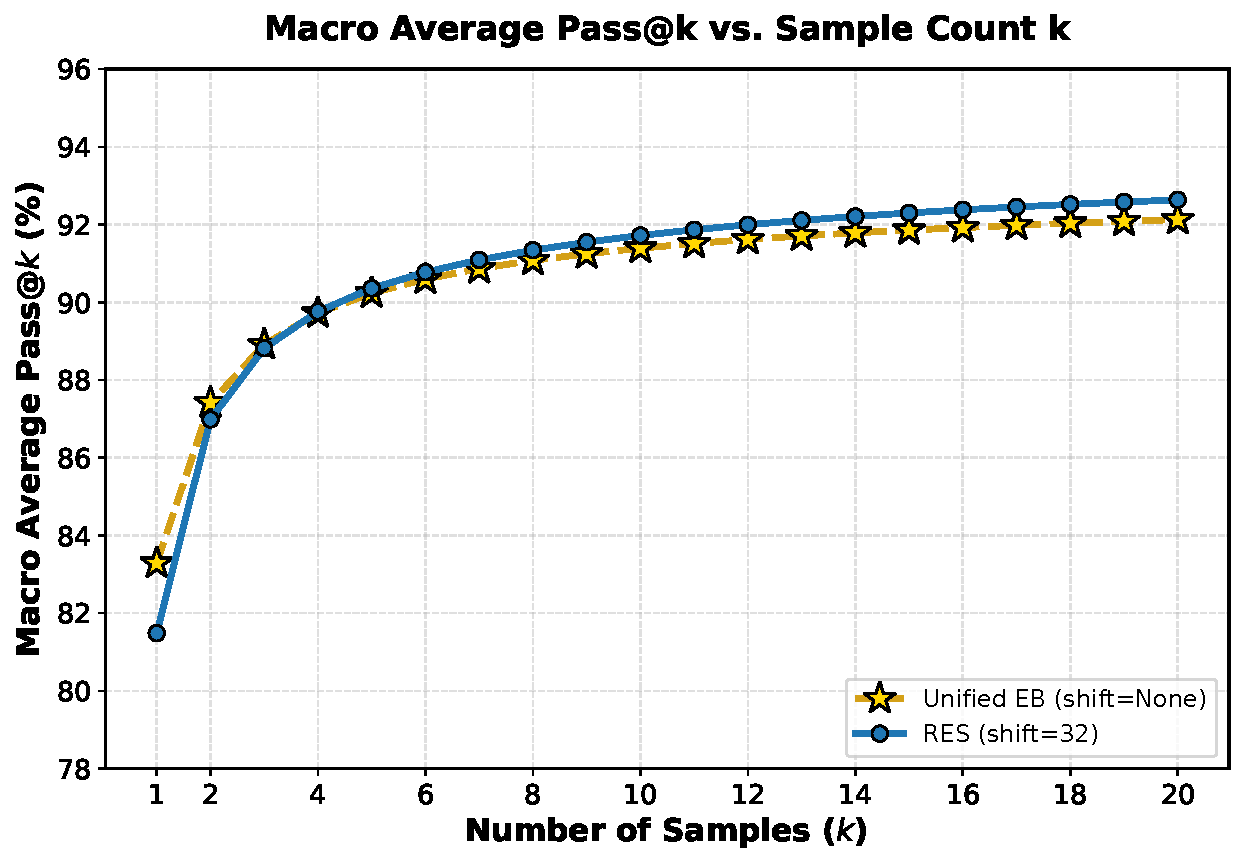
\includegraphics[width=\linewidth]{images/fig_macro_pass_at_k.pdf}
\captionof{figure}{\textbf{Macro Average Pass@$k$ vs.\ Sample Count $k$}. While Unified EB achieves higher Pass@1, RES ($s=32$) exhibits stronger multi-sample scaling, overtaking Unified EB at $k \ge 6$ and maintaining its advantage through $k=20$. Table~\ref{tab:eb_unified_vs_rolling} reports a 32.5\% increase in tokens per forward pass.}
\label{fig:macro_pass_at_k}

\end{minipage}
\par\vspace{12pt}
\begin{minipage}{\textwidth}
\centering
    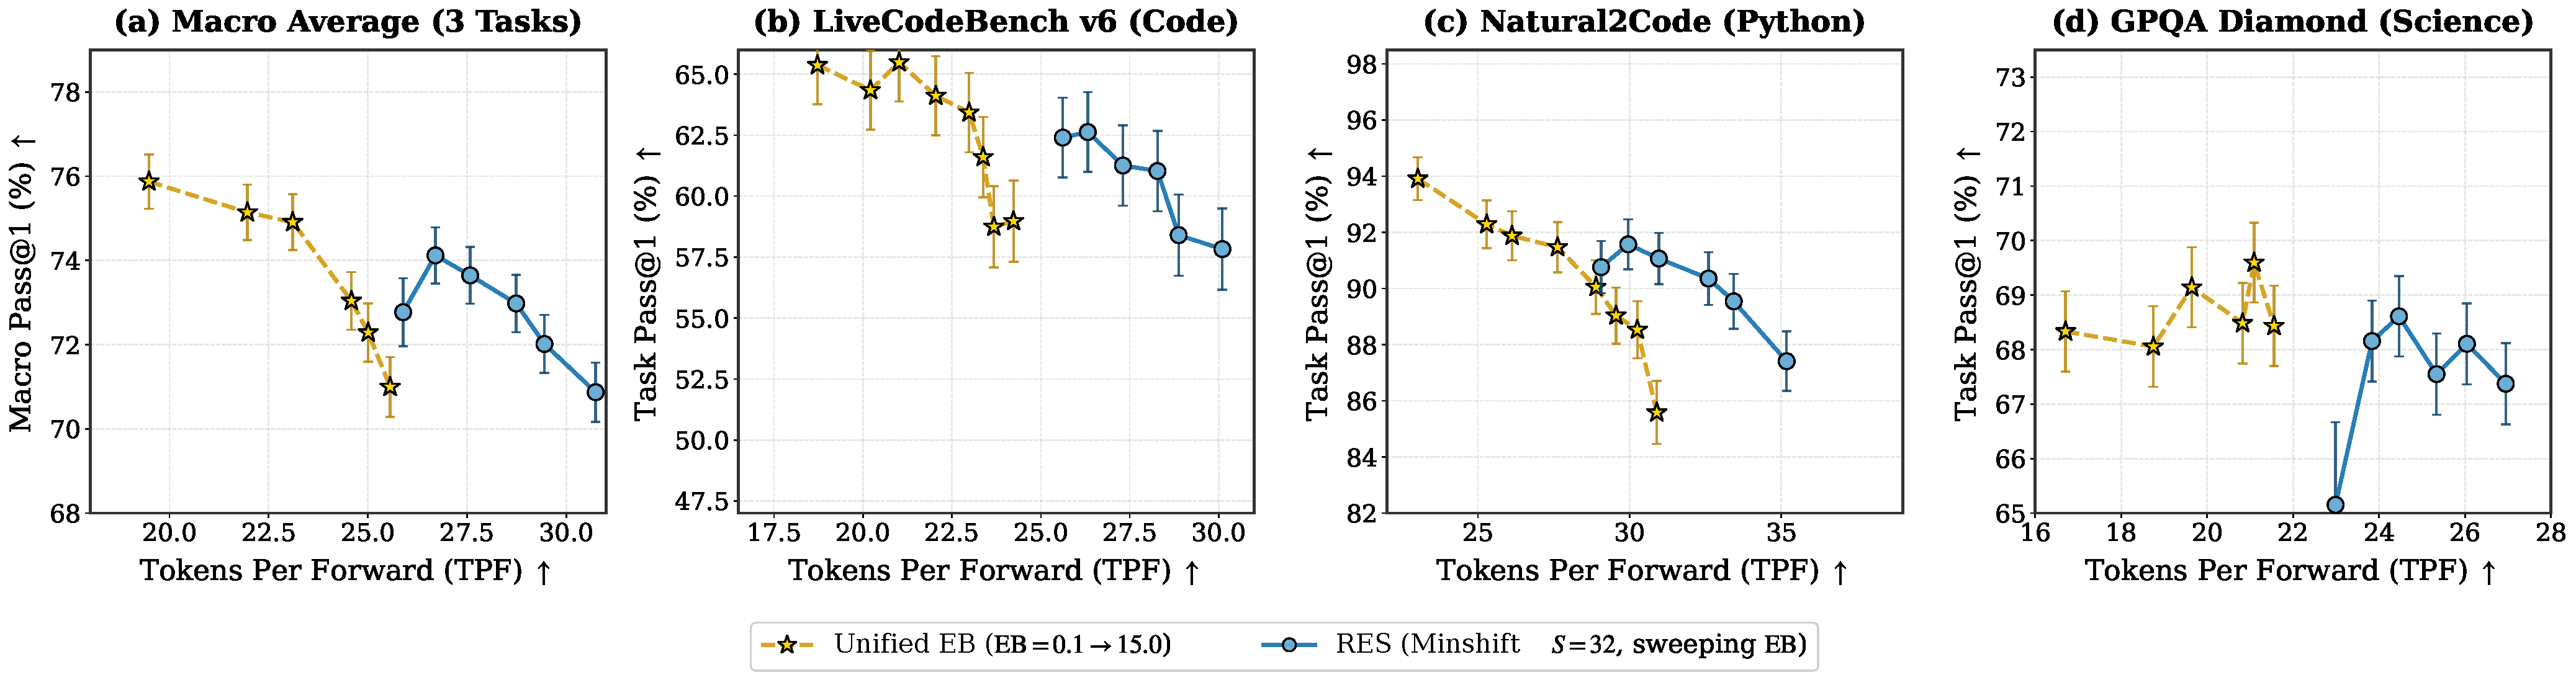
\includegraphics[width=\linewidth]{images/fig_merged_minshift32_eb01_1x4_row.pdf}
    \captionof{figure}{Pareto frontiers of RES with minimum shift $s=32$ and Unified EB under varied entropy bounds for LCB v6 and Natural2Code averaged over 5 seeds, and GPQA Diamond averaged over 20 seeds due to its higher evaluation variance.}
    \label{fig:minshift-16}

\end{minipage}
\end{minipage}
\end{lrbox}

\subsection{Main Results}
We compare RES against Unified EB on seven benchmarks at the default entropy bound $\gamma = 0.1$, averaging over 20 seeds (5 for LiveCodeBench).
Table~\ref{tab:eb_unified_vs_rolling} reports accuracy and tokens per forward pass (TPF).

\begin{figure}[tbp]
\centering
\usebox{\resultspanels}
\end{figure}


\paragraph{Performance and Efficiency}
RES raises TPF on every benchmark, by 23\% to 43\%, and \textbf{by 32.5\% on the macro average} (19.3 to 25.5).
Macro accuracy falls by 1.9 points, from 80.7\% to 78.8\%.
The cost is uneven across tasks.
Accuracy rises on MMLU ($+2.5$ points) and is unchanged within confidence intervals on GPQA Diamond; it falls by 0.5 to 2.8 points on GSM8k, HiddenMath, Natural2Code, and LiveCodeBench; and it falls by 10.7 points on IFEval, the one task where RES is clearly worse.
Excluding IFEval, the macro drop is 0.5 points.
One possible cause of the degradation is exposure bias: RES induces a noise pattern across the window that is heavily left-to-right, which is distinct from the homogeneous noise level used within the block at training time.
We do not test this explanation here.

\subsection{Speed-Quality Frontier}
We next sweep both knobs of RES, using the macro-average across LCB v6, GPQA Diamond, and Natural2Code.

\begin{figure}[tbp]
    \centering
    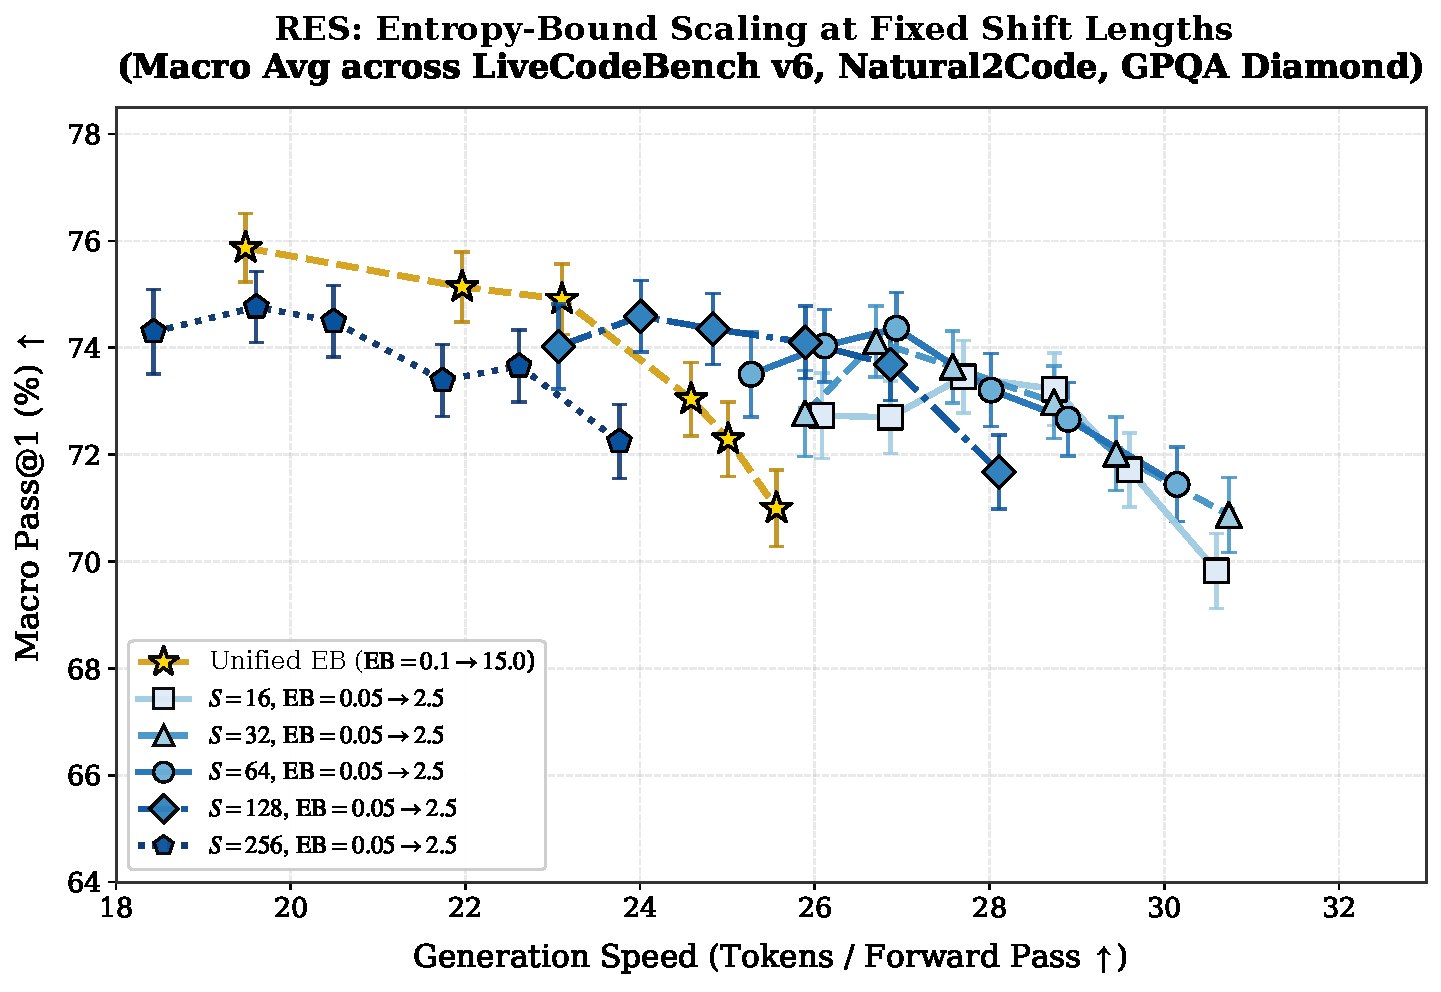
\includegraphics[width=0.6\linewidth]{images/fig_merged_minshift_by_eb_macro.pdf}
    \caption{Frontiers obtained by varying both the minimum shift $s$ in $F_{commit}$ (``S'' in the legend) and the entropy bound in $F_{route}$ for RES. Small shifts extend the frontier to higher throughput than Unified EB reaches.}
    \label{fig:dual-frontier}
\end{figure}


\paragraph{Entropy-Bound Sweep}
We sweep the entropy bound for RES with minimum shift $s=32$ and for Unified EB, and show the frontiers in Figure~\ref{fig:minshift-16}.
Relaxing the entropy bound alone takes Unified EB to about 25.5 TPF, where macro Pass@1 has fallen to about 71\%.
At a similar speed RES holds about 74\%, and it reaches the same 71\% only at about 31 TPF.
The gain is in the high-throughput regime: below about 23 TPF Unified EB remains the better choice, so RES extends the frontier rather than dominating it.

\paragraph{Minimum Shift Sweep}
While Unified EB has one axis to trade off performance and speed, RES has the minimum shift in addition to the entropy bound.
Figure~\ref{fig:dual-frontier} shows the frontier for each minimum shift.
Minimum shifts of 16 to 64 give similar frontiers, between about 26 and 31 TPF.
Larger shifts move the frontier toward lower throughput: $s=128$ covers about 23 to 28 TPF, and $s=256$ about 18 to 24 TPF.
This direction is expected: a larger minimum shift requires a longer accepted prefix before commitment, moving the decision toward the block level and retaining positions in the denoising window for more computation.
In this sweep the largest shift does not recover the accuracy of Unified EB at low throughput, so we recommend small shifts for the high-throughput regime and Unified EB otherwise.

\subsection{Multi-Sample Performance}
RES also scales better with the number of samples (Figure~\ref{fig:macro_pass_at_k}).
Unified EB has the higher Pass@1, but RES with $s=32$ overtakes it from $k \ge 6$ samples and maintains its advantage through $k=20$.
We hypothesize that the EB sampler avoids making ``difficult'' decisions, as it always accepts the lowest entropy positions first.
In contrast, the rolling mechanism along with the position-based temperature schedule enforces a left-to-right generation bias, which was shown in \citet{ni2026flexibility} to improve diversity across generations.
